%----------------------------------------------------------
\def\notedate{2022.11.04}
\def\currentauthor{Василян А.Р. (РК6-73Б)}
%----------------------------------------------------------
\notestatement{rndhpcgui}{Разработка web-приложения}

%---------------------------------------------------------
На рисунке ~\ref{picture1} представлено дерево проекта.
\begin{figure}[!ht]
  \centering
  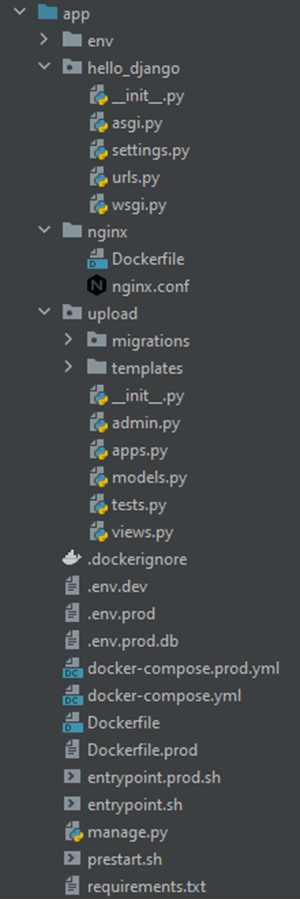
\includegraphics[scale=0.8]{ResearchNotes/rndhpc_not_gui_2022_11_04/picture1.png}
  \caption{Дерево проекта}
  \label{picture1}
\end{figure}

Была добавлена работа со статическими файлами и возможность загружать фотографию в контейнер и вывести на страницу (рисунок ~\ref{picture4}).

В новом \textsf{Dockerfile.prod} (листинг ~\ref{dockerfile.prod}) используется многоступенчатая сборка (\textsf{multi-stage build}) , чтобы уменьшить конечный размер образа. \textsf{builder} — это временный образ, которое используется для сборки \textsf{Python}. Затем он копируются в конечный производственный образ, а образ \textsf{builder} отбрасывается. Так же мы создали пользователя app без полномочий \textsf{root}. По умолчанию \textsf{Docker} запускает контейнерные процессы как \textsf{root} внутри контейнера, и если кто-то получит доступ на сервер и к контейнеру, то проникший на сервер пользователь тоже станет \textsf{root}, что, очевидно, не желательно. Таким образом увеличивается безопасность. Были созданы папки \textsf{staticfiles} и \textsf{mediafiles}, так как \textsf{docker-compose} монтирует именованные тома как \textsf{root}. И так как используется пользователь \textsf{app} не обладает полномочиями \textsf{root}, таким образом можно получить ошибку отказа в разрешении при запуске команды \textsf{collectstatic}, если каталог еще не существует.
	Так же был использован \textsf{Guncorn} (сервер промышленного уровня) и также добавлен в файл \textsf{requirements.txt} (версия \textsf{20.0.4}).

\begin{lstlisting}[frame=single, label={dockerfile.prod}, caption={Dockerfile.prod}, language={docker}] 
# BUILDER

FROM python:3.9.6-alpine as builder

# установка рабочей директории
WORKDIR /usr/src/app

# установка переменных окружения
ENV PYTHONDONTWRITEBYTECODE 1
ENV PYTHONUNBUFFERED 1

# установите зависимости psycopg2
RUN apk update \
    && apk add postgresql-dev gcc python3-dev musl-dev

RUN pip install --upgrade pip
RUN pip install flake8
COPY . .
#RUN flake8 --ignore=E501,F401 .

# установка зависимостей
COPY ./requirements.txt .
RUN pip wheel --no-cache-dir --no-deps --wheel-dir /usr/src/app/wheels -r requirements.txt

# FINAL

FROM python:3.9.6-alpine

# создание каталога для пользователя app
RUN mkdir -p /home/app

# создание пользователя app
RUN addgroup -S app && adduser -S app -G app

# создание необходимых директорий
ENV HOME=/home/app
ENV APP_HOME=/home/app/web
RUN mkdir $APP_HOME
RUN mkdir $APP_HOME/staticfiles
RUN mkdir $APP_HOME/mediafiles
WORKDIR $APP_HOME

# установка зависимостей
RUN apk update && apk add libpq
COPY --from=builder /usr/src/app/wheels /wheels
COPY --from=builder /usr/src/app/requirements.txt .
RUN pip install --no-cache /wheels/*

# копирование entrypoint.prod.sh
COPY ./entrypoint.prod.sh .
RUN sed -i 's/\r$//g'  $APP_HOME/entrypoint.prod.sh
RUN chmod +x  $APP_HOME/entrypoint.prod.sh

# копирование проекта в контейнер
COPY . $APP_HOME

# chown  файлам пользователя
RUN chown -R app:app $APP_HOME

# переход к пользователю app
USER app

# запуск entrypoint.prod.sh
ENTRYPOINT ["/home/app/web/entrypoint.prod.sh"]
\end{lstlisting}
	В \textsf{docker-compose.prod} (листинг ~\ref{docker-compose.prod }) был добавлен новый сервис \textsf{Nginx}, чтобы он действовал как обратный прокси-сервер для \textsf{Gunicorn} для обработки клиентских запросов, а также для обслуживания статических файлов. Для работы \textsf{Nginx} была создана новая директория с соответствующим названием. В данной директории были созданы файлы \textsf{Dockerfile} (листинг ~\ref{dockerfile_nginx}) и \textsf{nginx.conf} (листинг  ~\ref{nginx.conf}).

\begin{lstlisting}[frame=single, label={docker-compose.prod}, caption={docker-compose.prod.yml}, language={docker-compose}] 
version: '3.8'

services:
  web:
    build:
      context: ./
      dockerfile: Dockerfile.prod
    command: gunicorn hello_django.wsgi:application --bind 0.0.0.0:8000
    volumes:
      - static_volume:/home/app/web/staticfiles
      - media_volume:/home/app/web/mediafiles
    expose:
      - 8000
    env_file:
      - ./.env.prod
    depends_on:
      - db
  db:
    image: postgres:13.0-alpine
    volumes:
      - postgres_data:/var/lib/postgresql/data/
    env_file:
      - ./.env.prod.db
  nginx:
    build: ./nginx
    volumes:
      - static_volume:/home/app/web/staticfiles
      - media_volume:/home/app/web/mediafiles
    ports:
      - 1337:80
    depends_on:
      - web

volumes:
  postgres_data:
  static_volume:
  media_volume:
\end{lstlisting}

\begin{lstlisting}[frame=single, label={dockerfile_nginx}, caption={Dockerfile в директории nginx}, language={docker}] 
FROM nginx:1.21-alpine
RUN rm /etc/nginx/conf.d/default.conf
COPY nginx.conf /etc/nginx/conf.d
\end{lstlisting}

\begin{lstlisting}[frame=single, label={nginx.conf}, caption={nginx.conf}, language={nginx}] 
upstream hello_django {
    server web:8000;
}

server {
    listen 80;

    location / {
        proxy_pass http://hello_django;
        proxy_set_header X-Forwarded-For $proxy_add_x_forwarded_for;
        proxy_set_header Host $host;
        proxy_redirect off;
    }

    location /static/ {
        alias /home/app/web/staticfiles/;
    }

    location /media/ {
        alias /home/app/web/mediafiles/;
    }
}
\end{lstlisting}

	Для работы с медиафайлами был создан новый модуль \textsf{Django} под названием \textsf{upload}, то есть была создана новая директория \textsf{upload} (новый модуль создаётся командой в терминале: "\textsf{docker-compose exec web python manage.py startapp upload}") и добавлен новый модуль в \textsf{INSTALLED_APPS} в \textsf{settings.py}.
	В созданной директории был изменен файл views.py (листинг  ~\ref{views}), была создана папка для шаблонов "templates" и в ней был создан новый шаблон \textsf{upload.html} (листинг ~\ref{upload}). Так же был изменен файл \textsf{app/hello_django/urls.py} (литсинг ~\ref{urls}).

\begin{lstlisting}[frame=single, label={views}, caption={views.py}, language=Python] 
from django.shortcuts import render
from django.core.files.storage import FileSystemStorage


def image_upload(request):
    if request.method == "POST" and request.FILES["image_file"]:
        image_file = request.FILES["image_file"]
        fs = FileSystemStorage()
        filename = fs.save(image_file.name, image_file)
        image_url = fs.url(filename)
        print(image_url)
        return render(request, "upload.html", {
            "image_url": image_url
        })
    return render(request, "upload.html")
\end{lstlisting}

\begin{lstlisting}[frame=single, label={upload}, caption={\textsf{upload.html}}, language=HTML] 
{\% block content \%}
  <form action="{\% url "upload" \%}" method="post" enctype="multipart/form-data">
    {\% csrf_token \%}
    <input type="file" name="image_file">
    <input type="submit" value="submit" />
  </form>

  {\% if image_url \%}
    <p>File uploaded at: <a href="{{ image_url }}">{{ image_url }}</a></p>
    <img src="{{ image_url }}" alt="Your image will be placed here.">
  {\% endif \%}

{\% endblock \%}
\end{lstlisting}

\begin{lstlisting}[frame=single, label={urls}, caption={\textsf{urls.py}}, language=Python] 
from django.contrib import admin
from django.urls import path
from django.conf import settings
from django.conf.urls.static import static
from upload.views import image_upload

urlpatterns = [
    path("", image_upload, name="upload"),
    path("admin/", admin.site.urls),
]

if bool(settings.DEBUG):
    urlpatterns += static(settings.MEDIA_URL, document_root=settings.MEDIA_ROOT)
\end{lstlisting}

	Итак, командами представленными ниже запускаются контейнеры:
\textsf{docker-compose -f docker-compose.prod.yml up -d --build}
\textsf{docker-compose -f docker-compose.prod.yml exec web python manage.py migrate --noinput}
\textsf{docker-compose -f docker-compose.prod.yml exec web python manage.py collectstatic --no-input –clear}
	После запуска, при переходе по адресу \textsf{http://localhost:1337/}, открывается страница (рис. ~\ref{picture2}). Можно выбрать файл (рис.~\ref{picture3}). И после нажатия на \textsf{submit} страница обновляется, и теперь на ней присутствует ссылка на выбранное изображение, которое теперь сохранено в контейнере, и само изображение (рис. ~\ref{picture4}). Авторизация так же присутствует по адресу \textsf{http://localhost:1337/admin} аналогично тому, что было показано выше.

\begin{figure}[!ht]
  \centering
  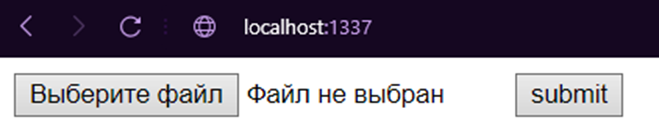
\includegraphics[scale=0.8]{ResearchNotes/rndhpc_not_gui_2022_11_04/picture2.png}
  \caption{Страница для загрузки фотографии}
  \label{picture2}
\end{figure}

\begin{figure}[!ht]
  \centering
  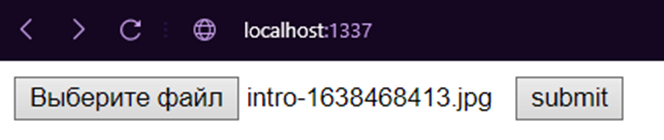
\includegraphics[scale=0.8]{ResearchNotes/rndhpc_not_gui_2022_11_04/picture3.png}
  \caption{Фотография выбрана}
  \label{picture3}
\end{figure}

\begin{figure}[!ht]
  \centering
  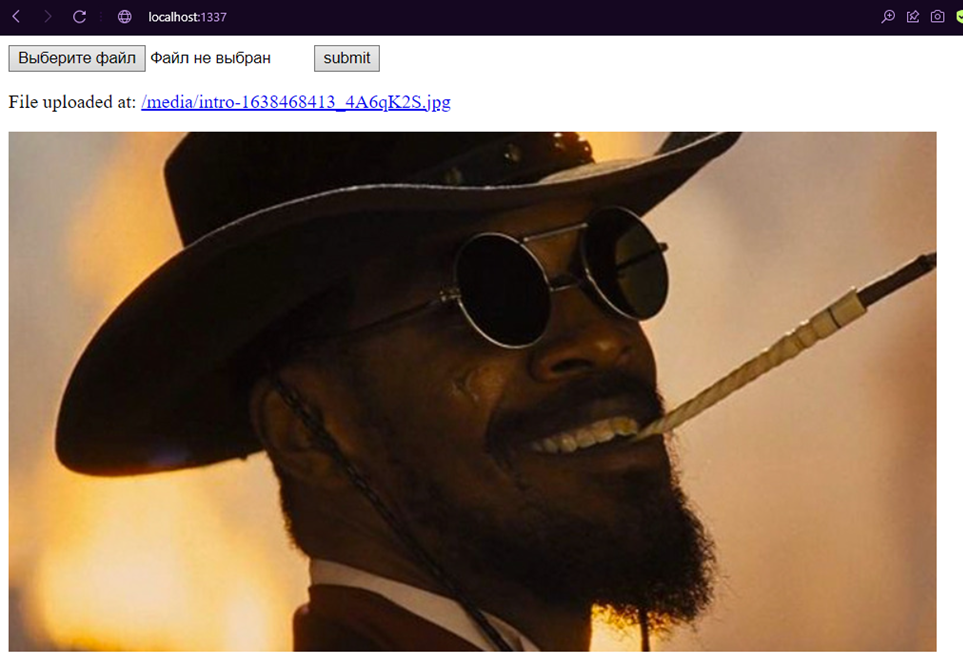
\includegraphics[scale=0.8]{ResearchNotes/rndhpc_not_gui_2022_11_04/picture4.png}
  \caption{Страница после нажатия на submit}
  \label{picture4}
\end{figure}
%----------------------------------------------------------
% Атрибуты задачи
\noteattributes{}
%----------------------------------------------------------
